\section{Introduction}\label{sec:intro}

Instructors of large introductory programming courses cannot read every failed submission, yet they would like to know what the class as a whole gets wrong so that they can re-teach it. A popular answer is to cluster failed submissions and to summarise each cluster for the instructor. In the most common formulation, each submission is an object described by attribute--value pairs that record which test cases it fails (an object--attribute--value, OAV, representation), the objects are clustered with K-means or a Hamming-distance method, and production rules of the form IF~\emph{symptom} THEN~\emph{misconception} are induced to explain the clusters. The appeal is clear: test outcomes are available in every autograder, the representation is interpretable, and the rules read like teaching advice.

Whether such clusters group submissions by the \emph{mechanism} of the error is rarely tested, for a simple reason: public datasets of failed programs do not come with mechanism labels, and asking experts to label thousands of programs is expensive and hard to reproduce. Without labels, cluster quality is judged by internal indices such as silhouette, or by the fidelity of surrogate rules to the clusters. Neither says whether two programs that fail the same tests fail them for the same reason.

\Cref{fig:example} makes the problem concrete. Of the {{example_total}} failing submissions to one assignment of our corpus, {{example_same}} fail all four tests, so a test-case OAV puts them in one cluster and any rule that reads it states one conclusion for all of them. The three programs in the figure need three different minimal repairs---a missing newline, a missing zero-padding specifier and a missing pair of parentheses---and their outputs deviate from the expected output in three different ways. What separates them is not the pass/fail vector but \emph{how} each output differs.

\begin{figure}[tbp]
\centering
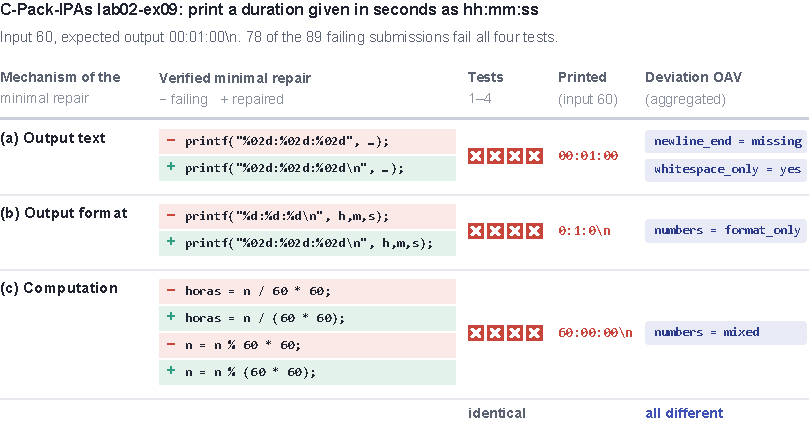
\includegraphics[width=\textwidth]{figures/fig1_example_en.pdf}
\caption{Three failing submissions to the same assignment (C-Pack-IPAs, anonymised) with an identical test signature. Their verified minimal repairs belong to three mechanism categories, and the aggregated deviation descriptors of \cref{sec:reps} differ for each of them. Long \texttt{printf} arguments are elided; the printed output is shown for the first test, with \texttt{\textbackslash n} for a newline.}\label{fig:example}
\end{figure}

This paper builds the missing evaluation data without new annotation and uses it to test the classic pipeline. Our starting point is that a student's own later submission often repairs the failed one. We replay a public corpus of {{n_submissions}} C90 submissions \citep{orvalho2024cpack} in an isolated runner, pair each failing submission with the same student's next passing submission, and use delta debugging to reduce their difference to a verified minimal repair, that is, the smallest set of changed lines that, applied to the failing program, makes it pass every test. A deterministic classifier assigns this repair to one of twelve program-level categories, from loop boundaries to output format. The labels are therefore grounded in executed evidence rather than in judgement, and every one of them can be re-derived. Because real repairs are imbalanced and often mix several changes, we add a second benchmark of controlled single-edit mutants of accepted programs whose category is known by construction. With these benchmarks we answer four research questions:
\begin{description}
\item[RQ1] How much mechanism information does the test-outcome OAV lose?
\item[RQ2] Do label-free descriptions of how the output deviates from the oracle recover mechanisms better at the same clustering budget?
\item[RQ3] Do IF--THEN rules induced with the Inductive Learning Algorithm (ILA) and its noise-tolerant variant ILA-2 \citep{tolun1998ila,tolun1999ila2} predict the mechanism of new students, and do they carry over to new assignments?
\item[RQ4] Do frozen neural code embeddings cluster failing programs by mechanism or by the program they derive from?
\end{description}
Each question is tied to registered hypotheses with falsification criteria (\cref{sec:hyp}); hypotheses, representations, weights and statistical rules were fixed before the evaluation, and every departure is recorded as a dated amendment. \Cref{fig:overview} gives an overview of the study.

\begin{figure}[tbp]
\centering
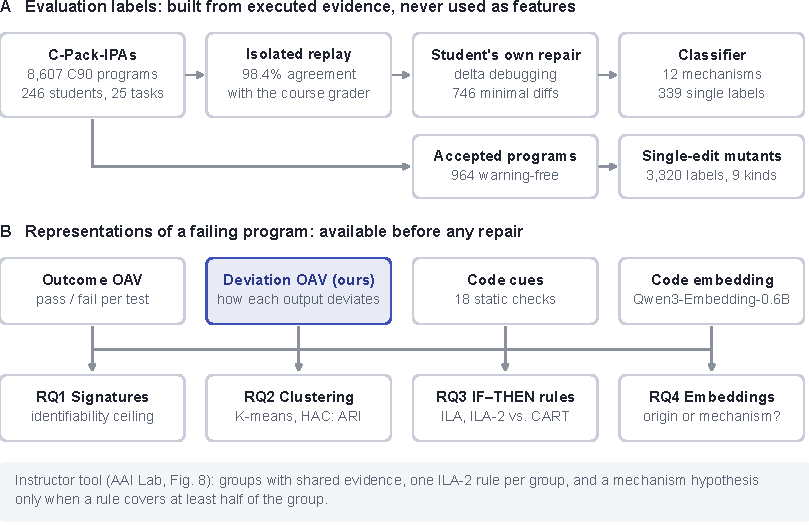
\includegraphics[width=\textwidth]{figures/fig2_overview_en.pdf}
\caption{Overview of the study. (A) Evaluation labels come from executed evidence: the student's own repair reduced by delta debugging, and single-edit mutants of accepted programs; they are never used as features. (B) Representations are computed from the failing program and its own runs only. The four research questions compare these representations against the labels, and the instructor tool of \cref{sec:tool} applies the resulting design.}\label{fig:overview}
\end{figure}

Our contributions are:
\begin{enumerate}
\item a reproducible, isolated replay of C-Pack-IPAs with an oracle audit against the historical grader ({{audit_cells_pct}}\% agreement over {{audit_cells}} test verdicts) and a second independent replay ({{repro_cells_pct}}\% agreement);
\item a repair-grounded benchmark built from {{n_pairs}} student repair events ({{real_ok}} verified pairs, {{n_real_gold}} single-mechanism labels) and a controlled benchmark of {{n_injected}} single-edit mutants, sharing one taxonomy and one classifier;
\item execution-deviation OAV, a label-free and problem-agnostic representation of output deviations, and an evaluation protocol with an identifiability ceiling and a granularity-matched null;
\item pre-registered evidence that test signatures mix mechanisms (at most {{real_H1a_pct}}\% of real and {{injected_H1a_pct}}\% of injected items are identifiable from them), that output-deviation evidence recovers mechanisms better on controlled data but not reliably on real repairs, that rules over it transfer to unseen assignments, and that a frozen code embedding clusters programs by origin;
\item an instructor tool that applies these findings: it groups a class's failing programs with the deviation OAV, attaches shared evidence and one induced rule to every group, and states a mechanism hypothesis only when a rule covers most of the group.
\end{enumerate}
We release the replay runner, benchmarks, protocol, analysis code and tool. Throughout, a label describes what changed in the program; it is not a claim about what the student believed. \Cref{sec:related} reviews related work, \cref{sec:data} builds the benchmarks, \cref{sec:methods} defines representations, analyses and hypotheses, \cref{sec:results} answers the research questions, \cref{sec:discussion} discusses implications and limitations, and \cref{sec:conclusion} concludes.
